\section{Bandwidth Reduction}

Gabriel applications continuously stream sensor data to the cloudlet. The richer
a sensing modality is, the more information can be extracted. Visual data from
cameras is one of such rich sensing modalities that wearable cognitive
assistance leverages. However, the last hop wireless bandwidth, especially LTE
bandwidth cannot support thousands of users simultaneously streaming high
definition videos. Therefore, to effectively scale wearable cognitive
assistance, we need to reduce the bandwidth consumed. There are three techniques
I will explore to reduce the bandwidth cost by exploiting the unique properties
of the workload. We have shown the effectiveness of these techniques with drone
footages. Further experiments with first-person videos will be done to show
their effectiveness for wearable cognitive assistance.

\subsection{Early Discard}
Early discard refers to the technique that filters and discards contents in
early stages of computation. An example system that uses early discard is an
unindexed search system~\cite{satyanarayanan2010searching}. In the mobile
computing context, ~\cite{hu2015case} explored using image-level simple computer
vision algorithms, for example blur and color detection, to suppress
transmission of uninteresting video frames.

In Gabriel applications, an efficient early discard system that filters out
uninteresting frames before transmission can reduce the bandwidth consumption.
For example, in the Lego assistant, all the assembled Lego pieces are placed on
a Lego board with black boundaries. Some frames do not contain the Lego board
due to user movement. Without further analysis, the application knows these
frames do not contain useful information since the board is not present. If an
efficient contour detection of black boundaries can be performed on the wearable
device, the application can save the unnecessary bandwidth consumed to transmit
the uninteresting frames.

There exists a tradeoff between computation and network transmission for early
discard. To one end, if the wearable device is powerful enough to perform all
the computation on-device within latency constraints, the bandwidth cost would
be minimal because there is no need to offload the computation. To the other
extreme, if the wearable device is very weak, all the sensor data then needs to
be shipped to the cloudlets for processing. In fact, image compression can be
thought as an early discard technique at the pixel level. It uses the
computation onboard to remove the duplicate data sent over the network.

To explore the effectiveness of early discard, we conducted experiments in a
small drone setting. Drones typically can carry more computational power than
wearable devices. Therefore they can be thought of futuristic wearable devices
with large computation capability. In my thesis, I will run similar experiments
on wearable devices with first-person videos. Below we will present our
experiments on drone videos to demonstrate the effectiveness of early discard.

\begin{figure*}
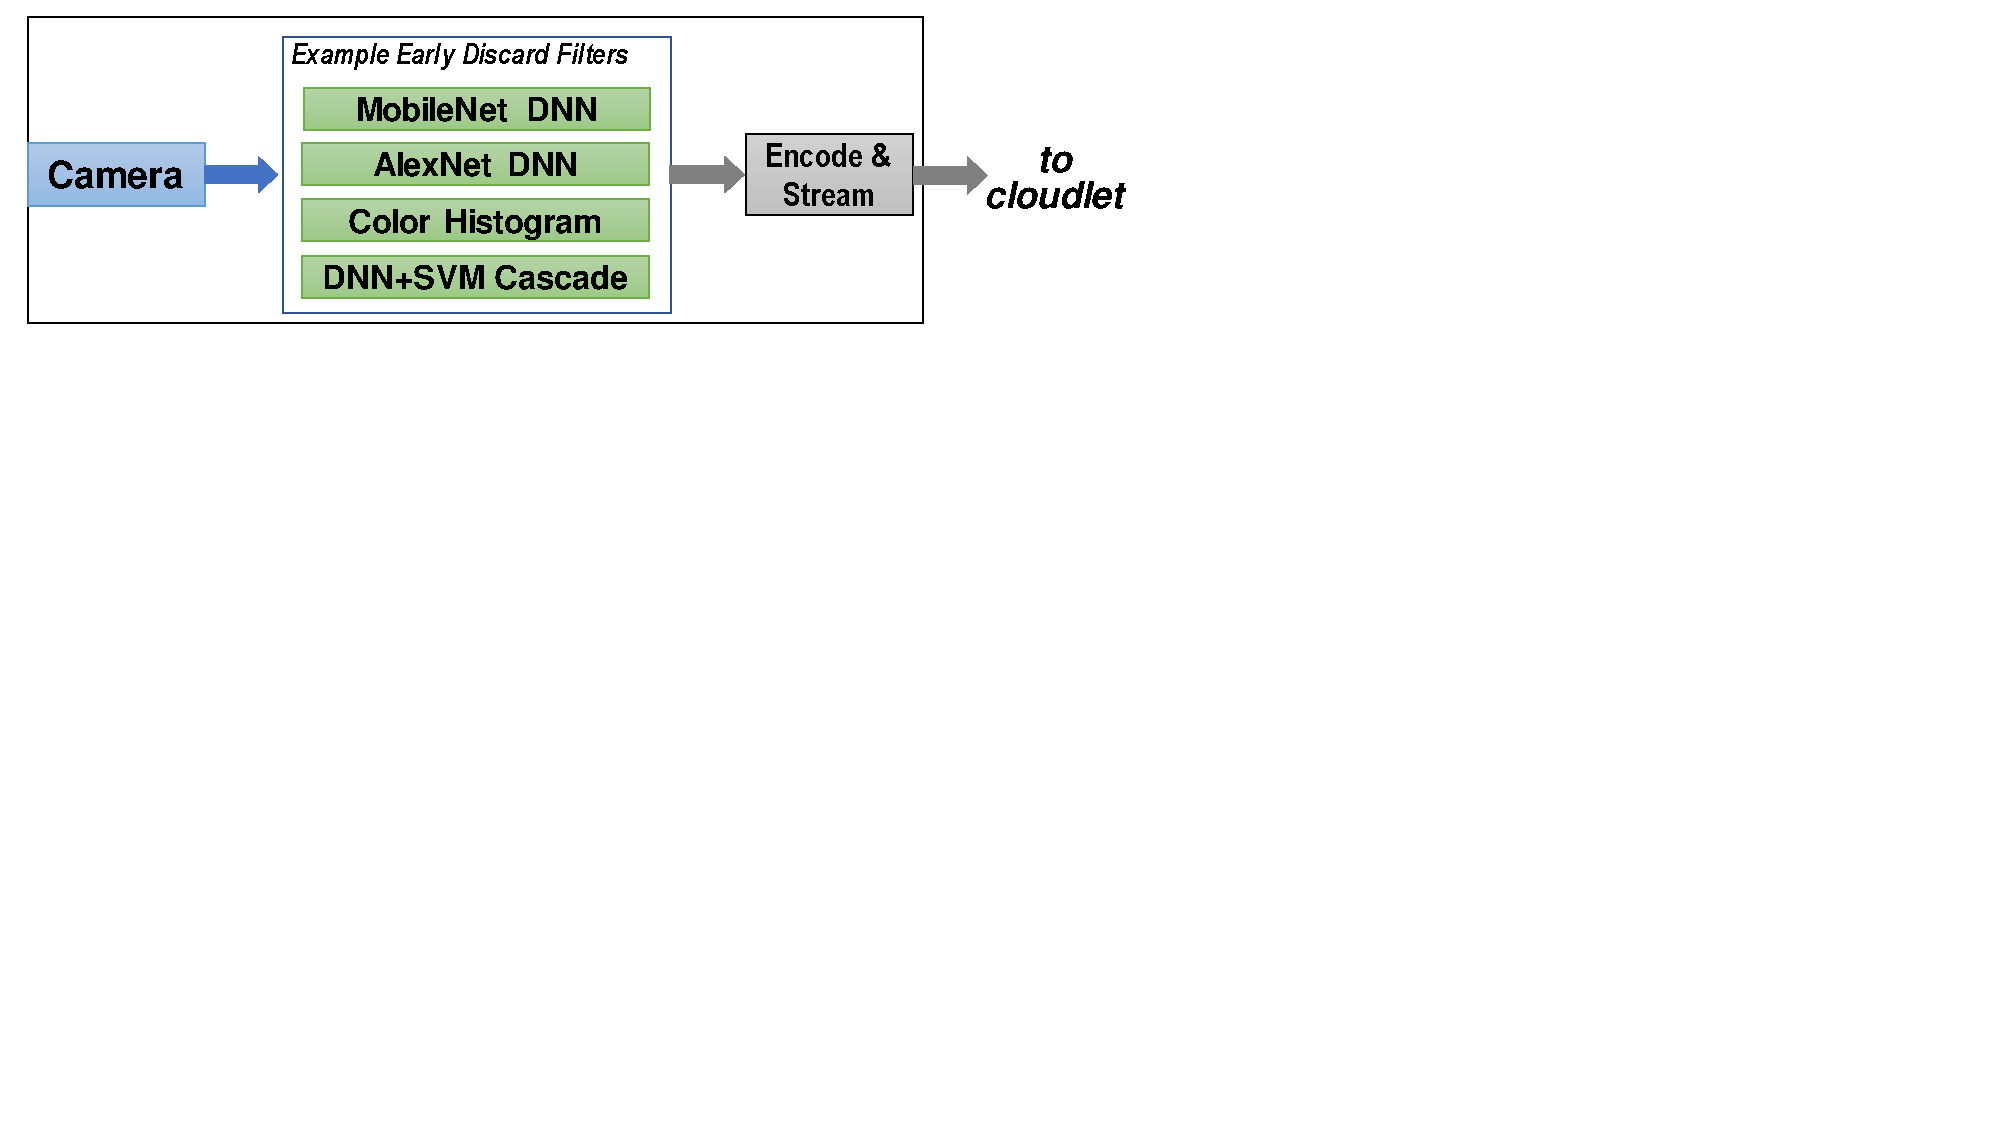
\includegraphics[scale=0.8,trim={0 13.5cm 10cm 0},clip]{FIGS/fig-early-discard.pdf}\\
\caption{Early Discard Pipeline.}
\label{fig:ondrone}
\vspace{-0.2in}
\end{figure*}


As shown in Figure~\ref{fig:ondrone}, we envision a choice of weak detectors
being available as early discard filters on a drone, with the specific choice of
filter being mission-specific. We use image classification as early discard
filters on the drone: it is not necessary to know exactly where in the frame a
relevant object occurs. This suggests that MobileNet would be a good choice as a
weak detector. Its speed of 352 ms per frame on Nexus 6 yields less than 3 fps.
However, its speed of 13 ms per frame on Jetson yields more than 75 fps. If
Jetson-class hardware was to be available on future smartphones, MobileNet
would be usable at a full frame rate. We therefore use MobileNet on the drone for
early discard in our experiments.

\begin{figure*}
\centering
\begin{tabular}{|p{1cm}|p{2cm}|p{2cm}|p{2.5cm}|p{2cm}|p{3cm}|}
\hline
   & Detection & Data & Data & Training & Testing \\ 
Task& Goal & Source & Attributes & Subset & Subset\\ 
\hline
T1 & {\small People in scenes of daily life}&{\small Okutama Action Dataset~\cite{Barekatain2017}}&\makecell[tl]{\small 33 videos \\\small 59842 fr\\\small 4K@30~fps}&\makecell[tl]{\small 9 videos\\\small 17763 fr}&\makecell[tl]{\small 6 videos\\\small 20751 frames}\\ 
\hline
T2 &{\small Moving cars}&{\small Stanford Drone Dataset~\cite{Robicquet2016}}&\makecell[tl]{\small 60 videos \\\small 522497 fr\\\small 1080p@30~fps}&\makecell[tl]{\small 16 videos\\\small 179992 fr} & \multirow{4}{*}{\parbox{3cm}{\centering\small 14 videos 92378 fr\\ Combination of videos from each dataset. T1's test uses a subset that do not have unlabeled human.}} \\ \cline{1-5}
T3 &{\small Raft in flooding scene}&{\small YouTube collection~\cite{YouTube1}}&\makecell[tl]{\small 11 videos \\\small 54395 fr\\\small 720p@25~fps}&\makecell[tl]{\small 8 videos\\\small 43017 fr} & \\ \cline{1-5}
T4 &{\small Elephants in natural habitat}&{\small YouTube collection~\cite{YouTube2}}&\makecell[tl]{\small 11 videos \\\small 54203 fr\\\small 720p@25~fps}&\makecell[tl]{\small 8 videos\\\small 39466 fr} & \\ \cline{1-5}
\hline
\end{tabular}
\vspace{0.2in}
\begin{captiontext}
fr = ``frames''\\
fps = ``frames per second''\\
No overlap between training and testing subsets of data
\end{captiontext}
\caption{Benchmark Suite of Video Traces}
\label{fig:benchmarksuite}
\end{figure*}

Our experiments on the {\xc EarlyDiscard} strategy used benchmark tasks suite
described in figure ~\ref{fig:benchmarksuite}. We used Nvidia Jetson TX2 as the
drone platform. We use both frame-based and event-based metrics to evaluate the
MobileNet filters. These experiments demonstrate that significant bandwidth
saving can be achieved while maintaining final detection accuracy through
interesting frames selection with filters running on the mobile device.

\begin{figure}
    \centering
    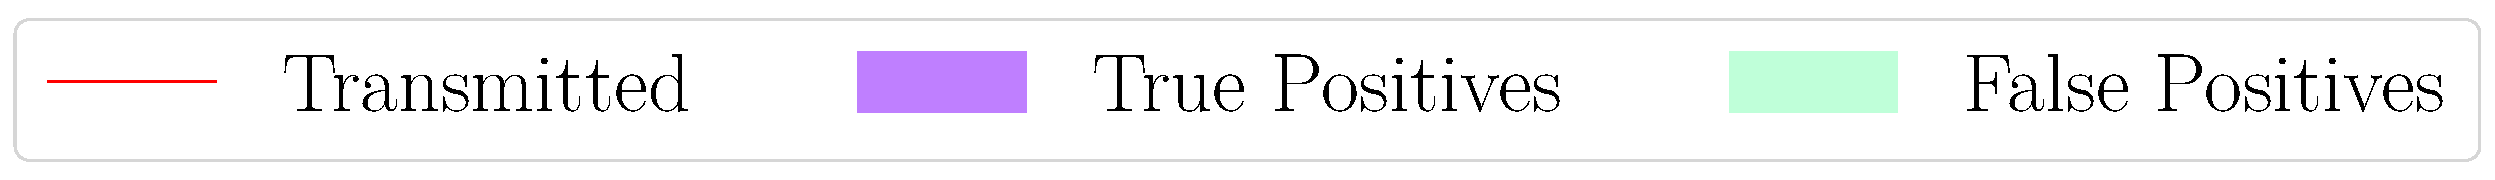
\includegraphics[width=0.9\linewidth]{FIGS/fig-event-recall-frame-percentage-legend.pdf}
    \hspace*{-0.35in}
    \begin{subfigure}[T1]{
        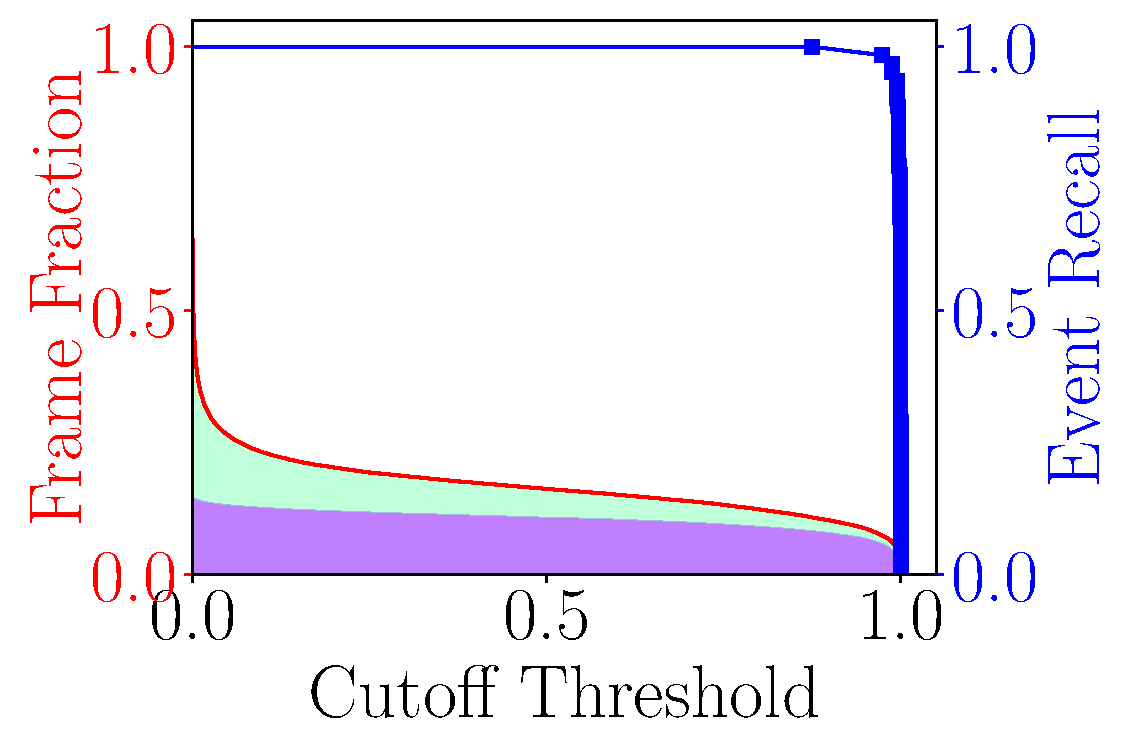
\includegraphics[width=0.4\linewidth]{FIGS/fig-event-recall-frame-percentage-vs-threshold-okutama.pdf}}        
    \end{subfigure}
    \begin{subfigure}[T2]{
      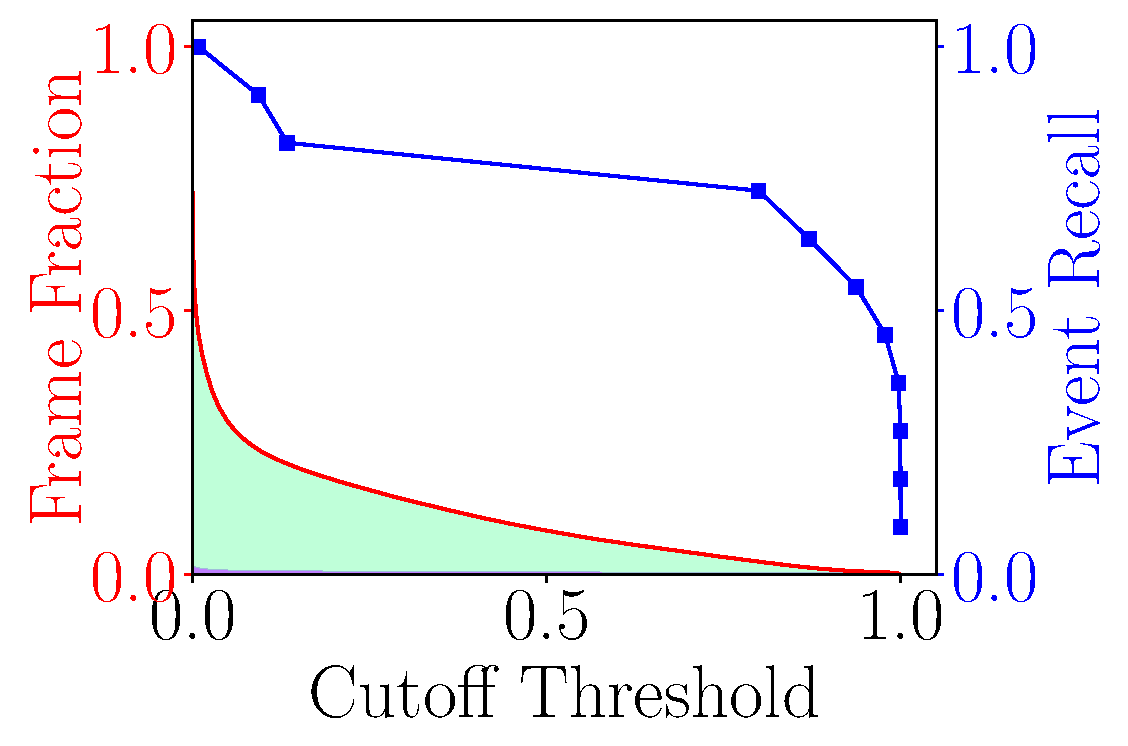
\includegraphics[width=0.4\linewidth]{FIGS/fig-event-recall-frame-percentage-vs-threshold-stanford.pdf}}
    \end{subfigure}
    \hspace*{-0.35in}    
    \begin{subfigure}[T3]{
      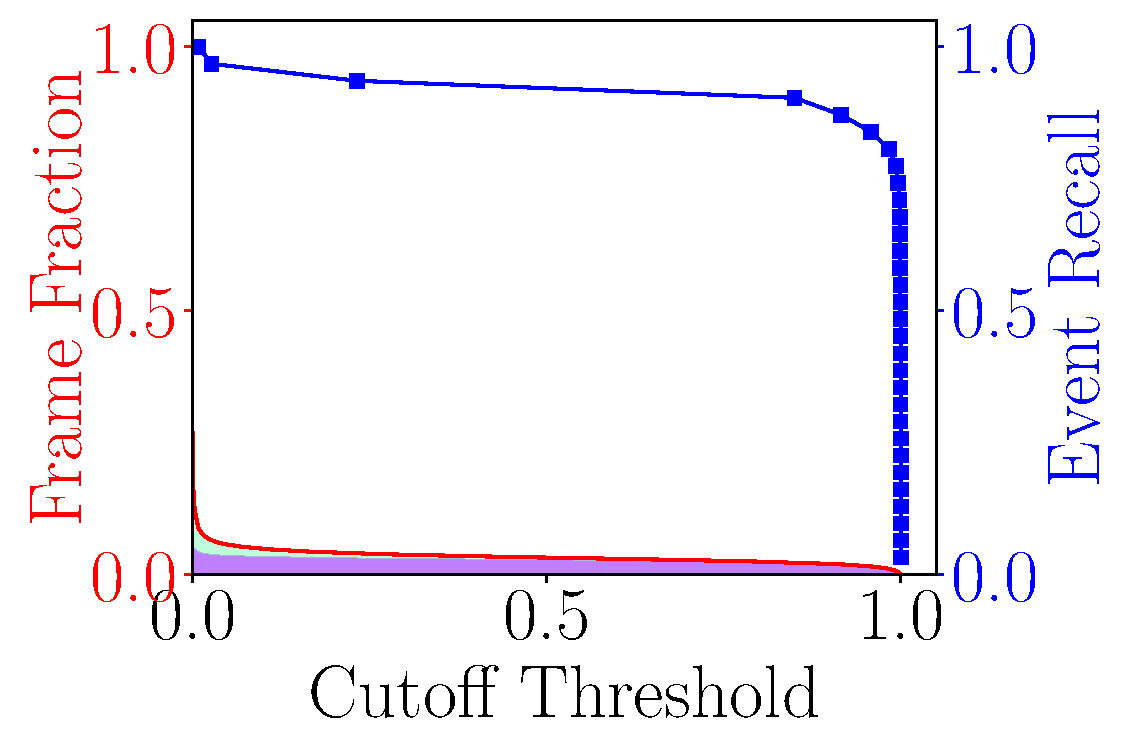
\includegraphics[width=0.4\linewidth]{FIGS/fig-event-recall-frame-percentage-vs-threshold-raft.pdf}}
    \end{subfigure}
    \begin{subfigure}[T4]{
      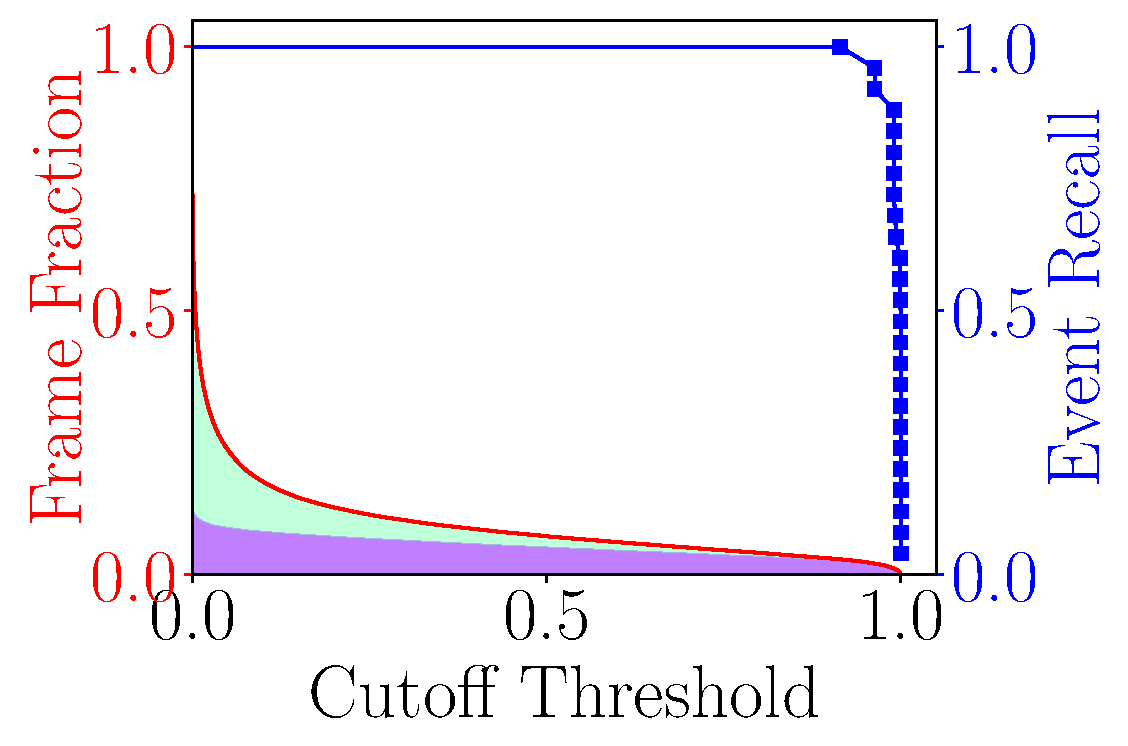
\includegraphics[width=0.4\linewidth]{FIGS/fig-event-recall-frame-percentage-vs-threshold-elephant.pdf}}
    \end{subfigure}
\vspace{-0.2in}
\caption{Where the Bandwidth Goes}
\label{fig:earlydiscard-frame-percent-breakdown}
\end{figure}

\noindent{\textbf{Drone Filter Accuracy}}: The output of a drone filter is the
probability of the current tile being ``interesting.''  A tunable {\em cutoff
  threshold} parameter specifies how interesting is ``interesting enough'' for
transmission to the cloudlet.  All tiles, whether deemed interesting or not,
are still stored in drone storage for post-mission processing.

Events (such as detection of a raft in T3) occur in consecutive frames, all of
which contain the object of interest. A correct detection of an event is
defined as at least one of the consecutive frames being transmitted to the
cloudlet.  Blue lines in Figure~\ref{fig:earlydiscard-frame-percent-breakdown}
shows how the event recalls of drone filters for different tasks change as a
function of cutoff threshold. As the figure shows, the MobileNet DNN filter is
able to detect all the events for T1 and T4 at a high cutoff threshold. For T2
and T3, the majority of the events are detected. Achieving high recall on T2
and T3 (on the order of 0.95 or better) requires setting a low cutoff
threshold.  This leads to the possibility that many of the transmitted frames
are actually uninteresting (i.e., false positives).

\noindent{\textbf{False negatives}}: As discussed earlier, false negatives are
a source of concern with early discard.  Once the drone drops a frame
containing an important event, improved cloudlet processing cannot help. The
results in the third column of Figure~\ref{fig:early-discard-results} confirm
that there are no false negatives for T1 and T4 at a cutoff threshold of 0.5.
For T2 and T3, lower cutoff thresholds are needed to achieve perfect recalls.

\begin{figure}
\centering
\begin{tabular}{|c|c|c|c|c|c|c|}
\hline
   &        &Dete-       &Avg&Total&Avg&Peak\\
   &Total&cted&Delay&Data&B/W&B/W\\
   &Events&Events&(s)&(MB)&(Mbps)&(Mbps)\\ 

\hline
\small
T1 & \phantom{0}62  & 100~\%       &  \phantom{0}0.1&\phantom{0}441  &  5.10     &   10.7  \\
\hline
T2 & \phantom{0}11  & \phantom{0}73~\%      & \phantom{0}4.9 & \phantom{00}13            &  0.03 & \phantom{0}7.0 \\ % 100% recall at 47% of frames, 82% recall at 21% of frames
\hline
T3 & \phantom{0}31  & \phantom{0}90~\%  & 12.7 & \phantom{00}93  &  0.24 &  \phantom{0}7.0 \\ % 100% recall at 9% frames
\hline
T4 & \phantom{0}25  & 100~\%       & \phantom{0}0.3 & \phantom{0}167  &  0.43 &  \phantom{0}7.0 \\
\hline
\end{tabular}\\
\caption{Recall, Event Latency and Bandwidth at Cutoff Threshold 0.5}
\label{fig:early-discard-results}
\end{figure}

\noindent{\textbf{Result latency}}: The contribution of early discard processing
to total result latency is calculated as the average time difference between the
first frame in which an object occurs (i.e., first occurrence in ground truth)
and the first frame containing the object that is transmitted to the backend
(i.e., first detection). The results in the fourth column of
Figure~\ref{fig:early-discard-results} confirm that early discard contributes
little to result latency. The amounts range from 0.1~s for T1 to 12.7~s for T3.
At the times cale of human actions such as dispatching of a rescue team, these
are negligible delays.

Although the general approach of early discard would apply for wearable
cognitive assistance, how to apply this technique to wearable devices still
needs investigation. First, wearable devices in general have even less
general-purpose computation capabilities. Due to the small form factor and heat
dissipation constraints, the mobile CPUs in wearable devices are optimized for
power instead of performance. In fact, many smart glasses today rely on a user's
smartphone to process information. For instance, one of Google Glasses' main use
cases when it was first released is to display notifications from smartphone
applications, such as CNN and EverNote~\cite{theverge2013}. Second, there is a
strong trend to put hardware DNN accelerators into embedded devices to perform
some analysis of visual data. There are many efforts from both industry and
academia. For example, Microsoft HoloLens has a special Holograhic Processing
Unit~\cite{theregister2016} to map the environment in 3D. Recently released
Google Pixel 2 smartphone have visual cores built-in for future-proofing although
not all of them are being actively used now~\cite{androidcentral2017}. In
academia, there are strong interests in DNN compression and optimization for
embedded devices so that the inference can run natively on
device~\cite{han2015deep}~\cite{han2016eie}. Therefore, it is likely that smart
glasses' computation capabilities, especially their capabilities of executing
DNNs, would vary greatly.

I would like to further explore how to create filters for a variety of
heterogeneous smart glasses with or without accelerators in my thesis. I plan to
formulate the problem as an optimization problem that optimizes for the least
amount of bandwidth consumption constraint by the application latency requirement.
To its simplistic form, the problem can be written as
\begin{equation*}
\begin{aligned}
& \text{minimize} & & AverageDataTransmittedPerImage \\
& \text{subject to} 
  & & OnBoard Processing Time \\
  & & & + Network Transmission Time \\
  & & & + Server Computation Time \leq Application Latency Requirement 
\end{aligned}
\end{equation*}
I also plan to design tools that will generate filters given these constraints.

\subsection{Just-in-time Learning}
Just-in-time-learning (JITL) refers to the technique that tunes the processing
pipeline to the characteristics of the current scenario in order to reduce
transmitted false positives from the client, therefore reduce wasted bandwidth.
When training DNNs to recognize and detect objects, machine learning experts do
their best to obtain training examples from the same distribution of the test
data. In other words, best efforts are made to acquire training examples from
environments similar to test environment in terms of lighting, occlusion, and
many other aspects. However, as a Gabriel application could be used in any
environment, it is not realistic to assume all of them can be truthfully
represented by the training data. For test environment that does not look
similar to the training environment, the detection accuracy could be lower.
Just-in-time-learning aims to alleviate the generalization problem by making
each test environment represented in the training samples. Such goal can be
achieved by quick collecting a small number of examples drawn from the actual
test environment and iteratively training an existing model with the newly
collected data in a short time.

I plan to focus on mechanical assembly tasks when applying just-in-time learning
to wearable cognitive assistance. For mechanical assembly tasks, the environment
a user is in usually does not change significantly. For example, a user might
sit in front of a desk for most of the time. The relatively stable environment gives
us opportunities to leverage the human in the loop to provide false positive
examples. Before the application starts, a cognitive assistant could ask the
user to look around her environment with the assembly kits put away for a short
period of time. By construction, any positive predictions are false positives.
They are excellent negative training examples because they are taken in the
actual test environment. I plan to explore multiple methods to make use of these
newly collected data. First, feature matching could be used to identify
subsequent false positives. Specifically, a false positive feature pool can be
built for the particular test environment with the newly collected negative
data. For each prediction at application runtime, a matching is performed to see
if it is close enough to items in the false positive feature pool. Second,
researchers have shown positive results from train image segmentation DNNs with
a small number of examples for a few iterations to fit the model better to the
test environment. I plan to explore similar techniques in object detections.

\subsection{Context-awareness}

The essence of this approach is to leverage unique attributes of the current
task to improve the speed and accuracy of image processing on the mobile device.
By definition, this approach is ad hoc in character. However, the wins can be
significant. Consider the fuchsia colored screw in RibLoc cognitive assistant as
an example. Since the color of the screw is rarely seen in everyday objects,
cheap color filtering instead of DNNs can be used to filter interesting frames.

%% searching for survivors in the
%% ocean after a shipwreck.  Suppose the standard approach for detecting
%% survivors in search and rescue missions involves detection of human
%% faces and bodies~(similar to T1), or distinctive actions such as
%% waving.  These are used as the basis of early discard
%% at the beginning of the mission.  During the mission, as personnel
%% review results that are presented to them after cloudlet processing,
%% they notice that all survivors are wearing flotation devices
%% (lifejackets) that have a distinctive color.  Against the
%% blue-green background of the ocean, detecting this color is a fast,
%% accurate, and computationally cheap way of detecting survivors.
%% Figure~\ref{fig:shipwreck}(a) gives an example of such a scene.
%% However this optimization is unique to this mission.  On a different
%% mission that also involves a shipwreck, the lifejackets may be of a
%% different color.  Or, because of the late afternoon timing of the
%% mission and the consequent low angle of the sun, too many false
%% positives may arise from reflections off the water if reddish-orange colors
%% are used as the basis of early discard.

%% \begin{figure}
%% \centering
%% 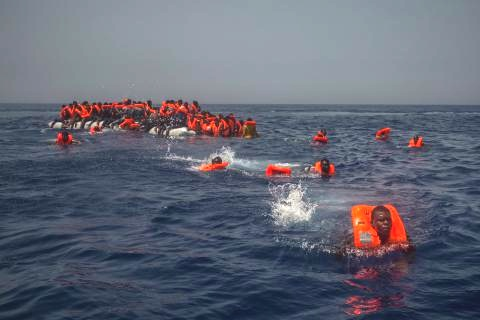
\includegraphics[width=2.5in]{FIGS/fig-shipwreck6.jpg}\\
%% (a) Motivating Image\\[0.2in]
%% \caption{Example of Context-Aware Strategy}
%% \label{fig:shipwreck}
%% \vspace{-0.2in}
%% \end{figure}


%% By the classic metrics of machine learning, the use of such heuristics
%% is viewed as ``overfitting'' and therefore something to be avoided at
%% all costs.  Yet, in practical terms and in the narrow context of this
%% mission, the heuristic offers many advantages without compromising
%% accuracy.  On some missions, the heuristic may even prove to be more
%% accurate than a DNN.  We consider it important to allow mission
%% personnel to take advantage of such context-aware optimizations.

%% Mission personnel can specify parameters to early filters by example. This can
%% done by drawing bounding boxes around the relevant parts of images that were
%% presented after cloudlet processing. Filters can be selectively activated or
%% deactivated, and combined to generate complex search predicates. They can be
%% used on the drone both for early discard of future video, as well as
%% re-examination of stored video. When the accuracy of the uploaded filter is
%% better than that of the default DNN filter, a re-examination of stored video can
%% yield hits that were missed earlier. These new hits can be downloaded to the
%% cloudlet for further processing. The context-aware filter is thus being used
%% both for reachback from already-captured video, as well as for early discard on
%% future video.

To demonstrate the effectiveness of this strategy, we apply it in the drone
context using a simple color filter in T3. In each raft search video, we
randomly pick a frame that contains a raft (true positive), and obtain the color
of the most distinctive region of the raft. Using the hue, saturation, and value
(HSV) color space attributes of this region, we apply a color filter to all the
other frames of the video. If a significantly large area of a frame passes this
filter, the frame is marked as positive. Otherwise, it is marked as negative.

\begin{figure}
\centering

\begin{tabular}{|l|l|l|l|}
\hline
        & \begin{tabular}[c]{@{}l@{}}Precision using\\ DNN (\%)\end{tabular} & \begin{tabular}[c]{@{}l@{}}Precision using\\ color filter (\%)\end{tabular} & \begin{tabular}[c]{@{}l@{}}Recall\\ (\%)\end{tabular} \\ \hline
Video 1 & 92.4                                                               & 95.3                                                                        & 89.1                                                  \\ \hline
Video 2 & 51.9                                                               & 76.1                                                                        & 90.0                                                  \\ \hline
Video 3 & 41.3                                                               & 84.3                                                                        & 88.6                                                  \\ \hline
\end{tabular}\\[0.1in]

(a) Accuracy\\[0.1in]

\begin{tabular}{|l|l|l|l|l|l|l|}
\hline
\multirow{2}{*}{} & \multicolumn{2}{c|}{Jetson} & \multicolumn{2}{c|}{Joule}   & \multicolumn{2}{c|}{Nexus 6}   \\ \cline{2-7}
                  & DNN                 & Color & DNN                  & Color & DNN                  & Color \\ \hline
Video 1           & \multirow{3}{*}{13} & 6.2   & \multirow{3}{*}{37} & 9.8   & \multirow{3}{*}{352} & 27.5  \\ \cline{1-1} \cline{3-3} \cline{5-5} \cline{7-7}
Video 2           &                     & 6.3   &                      & 9.7   &                      & 26.3  \\ \cline{1-1} \cline{3-3} \cline{5-5} \cline{7-7}
Video 3           &                     & 9.5   &                      & 12.3  &                      & 36.1  \\ \hline
\end{tabular}\\[0.1in]

(b) Processing time (ms)\\
\caption{Detection Results on T3 Using Color Filters}
\label{fig:colorfilter-results}
\vspace{-0.2in}
\end{figure}

Figure~\ref{fig:colorfilter-results} shows the results of using this
approach on three representative videos in T3.  Keeping recall fixed
at a high value (fourth column of
Figure~\ref{fig:colorfilter-results}(a)), the second and third columns
show the precision achieved using a DNN and a color filter.  For all
three videos, the precision using a color filter is better than the
precision using a DNN.  The difference is modest for Video 1, but
considerable for Video 2 and Video 3.  In other words, the context
aware approach is consistently more accurate.  This improvement in
accuracy does not come at a sacrifice in speed.  On the contrary,
Figure~\ref{fig:colorfilter-results}(b) shows that the DNN on the
Jetson takes 2--3 times the processing time of the color filter.  On
the Joule and the Nexus 6, it takes 8--10 times.  These results show
the high value of using context-aware knowledge.  What the DNN
provides is generality, combined with reasonable accuracy.  At the
beginning of a mission, when little is known about the
context-specific search attributes of the target, the DNN is the only
choice.  As the mission progresses, the early results may hint at the
attributes of a highly effective and cheap context-aware filter.

Although Gabriel applications do not have a human in the loop to specify filter
parameters, context-awareness can still be applied to wearable cognitive
assistance. In fact it could serve both as a mean to reduce bandwidth
consumption and as a method to reduce server computation latency. To achieve the
former goal, we can generate a suite of early-discard filters at training time
using different algorithms. When the application first starts, we can ask the
user to look around her environment and show us a few objects that will be used.
All early-discard filters can be evaluated during this ``warm-up'' time by
checking how many false positives and false negatives they produce. A filter
that performs the best in this test environment will be selected for application
usage. To be able to achieve such context-awareness, many challenges exist,
e.g. what metrics to use to evaluate these early discard filters, how to quickly
identify the best one to use, where should the computation happen, and how to
efficiently transmit context-aware updates to the client. I plan to explore
these questions in my thesis. In addition, such dynamic selection of CV
algorithms can be applied for processing at the edge nodes as well. We could
build upon the multi-algorithm acceleration approach described
by~\cite{chen2017empirical} to dynamically select a cheap algorithm to use from
auto-generated models in order to reduce processing latency.
